\documentclass[14pt]{extarticle}
% \documentclass[14pt]{article}

% \usepackage[style=authoryear,maxbibnames=9,maxcitenames=2,uniquelist=false,backend=biber,doi=false,url=false]{biblatex}
% \addbibresource{$BIB} % bibtex location
% \renewcommand*{\nameyeardelim}{\addcomma\space} % have comma in parencite
\usepackage{natbib}

\usepackage{xcolor}
\usepackage{amsmath}
\newcommand{\tuple}[1]{ \langle #1 \rangle }
%\usepackage{automata}
\usepackage{times}
\usepackage{ltablex}
\usepackage{tasks}

%%%%%% Template
\usepackage{hyperref}
\hypersetup{colorlinks=true,allcolors=blue}

\usepackage{vmargin}
\setpapersize{USletter}
\setmarginsrb{1.0in}{1.0in}{1.0in}{0.6in}{0pt}{0pt}{0pt}{0.4in}

% HOW TO USE THE ABOVE:
%\setmarginsrb{leftmargin}{topmargin}{rightmargin}{bottommargin}{headheight}{headsep}{footheight}{footskip}
%\raggedbottom
% paragraphs indent & skip:
\parindent  0.3cm
\parskip    -0.01cm

\usepackage{tikz}
\usetikzlibrary{backgrounds}

% hyphenation:
% \hyphenpenalty=10000 % no hyphen
% \exhyphenpenalty=10000 % no hyphen
\sloppy

% notes-style paragraph spacing and indentation:
\usepackage{parskip}
\setlength{\parindent}{0cm}

% let derivations break across pages
\allowdisplaybreaks

\newcommand{\orange}[1]{\textcolor{orange}{#1}}
\newcommand{\blue}[1]{\textcolor{blue}{#1}}
\newcommand{\red}[1]{\textcolor{red}{#1}}
\newcommand{\freq}[1]{{\bf \sf F}(#1)}
\newcommand{\datafreq}[2]{{{\bf \sf F}_{#1}(#2)}}

\def\qqquad{\quad\qquad}
\def\qqqquad{\qquad\qquad}

%%%%%%%%%%%%%%%%%%%%%%%%%%%%%%%%%%%%%%%%%%%%%%%%%%%%%%%%%%%%%%%%%%%%%%%%%%%%%%%%
%%%%%%%%%%%%%%%%%%%%%%%%%%%%%%%%%%%%%%%%%%%%%%%%%%%%%%%%%%%%%%%%%%%%%%%%%%%%%%%%

% fill-in-blank question style, found in https://tex.stackexchange.com/a/505089

\usepackage{ifthen}
\usepackage{tocloft}
\usepackage{exercise}
% \usepackage{xcolor}

% Set the Show Answers Boolean
\newboolean{showAns}
\setboolean{showAns}{false}
\newcommand{\showAns}{\setboolean{showAns}{true}}

% The length of the Answer line
\newlength{\answerlength}
\newcommand{\anslen}[1]{\settowidth{\answerlength}{#1}}

% ans command that indicates space for an answer or shows the answer in red
\newcommand{\ans}[1]{\settowidth{\answerlength}{\hspace{2ex}#1\hspace{2ex}}%
    \ifthenelse{\boolean{showAns}}%
        {\textcolor{red}{\underline{\hspace{2ex}#1\hspace{2ex}}}}%
        {}}%

\newcommand{\details}[1]{\settowidth{\answerlength}{#1}%
    \ifthenelse{\boolean{showAns}}%
        {\\ \textcolor{blue}{#1}}%
        {}}%

% Formatting how multiple choices Questions are formated.
\settasks{label=(\Alph*), label-width=30pt}


% Some commands for the Exercise Question package
\renewcommand{\QuestionNB}{\Large\protect\textcircled{\small\bfseries\arabic{Question}}\ }
\renewcommand{\ExerciseHeader}{} %no header
\renewcommand{\QuestionBefore}{3ex} %Space above each Q
\setlength{\QuestionIndent}{8pt} % Indent after Q number


% To create the list of answers with tocloft...
\newcommand{\listanswername}{Answers}
\newlistof[Question]{answer}{Answers}{\listanswername}

% Creates a TOC for Answers
\newcounter{prevQ}
\newcommand{\answer}[1]{\refstepcounter{answer}%
\ans{#1}%
\ifnum\theQuestion=\theprevQ%
        \addcontentsline{Answers}{answer}{\protect\numberline{}#1}% don't include the Q number
        \else%
        \addcontentsline{Answers}{answer}{\protect\numberline{\theQuestion}#1}%
        \setcounter{prevQ}{\value{Question}}%
        \fi%
        }%


%tocloft formatting listofanswers
\renewcommand{\cftAnswerstitlefont}{\bfseries\large}
\renewcommand{\cftanswerdotsep}{\cftnodots}
\cftpagenumbersoff{answer}
\addtolength{\cftanswernumwidth}{10pt}


%%%%%%%%%%%%%%%%%%%%%%%%%%%%%%%%%%%%%%%%%%%%%%%%%%%%%%%%%%%%%%%%%%%%%%%%%%%%%%%%
%%%%%%%%%%%%%%%%%%%%%%%%%%%%%%%%%%%%%%%%%%%%%%%%%%%%%%%%%%%%%%%%%%%%%%%%%%%%%%%%
\begin{document}

% \setcounter{section}{}
\centerline{\huge\bf ECON 2002.01 Problem Set 1}
\medskip
\centerline{\LARGE Unit 1 and Unit 2}
\medskip
\centerline{\LARGE Hui-Jun Chen}

\medskip

\showAns
\listofanswer


\begin{Exercise}

\Question The GDP in current US\$ for selected countries and the world are given below in \$ billions (source: World Bank). Based on this information, which of the following statements is correct?
\answer{B}

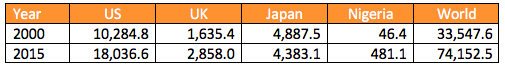
\includegraphics[width=\textwidth]{../QuestionBankImage/OUP-U1-Q1-01.png}

\begin{tasks}(1)
    \task The GDP of Japan grew by 10.3\% over the 15 years.
        \details{The GDP in Japan fell by 10.3\% over the 15 years.}
    \task Of the four countries, Nigeria was the only country that had a higher growth rate than that of the world over the 15 years.
        \details{GDP in each country grew by: US 75.4\%; UK 74.8\%; Japan -10.3\%; Nigeria 936.9\%; and the world 121.0\%.}
    \task The UK GDP growth rate was higher than that of the US.
        \details{The US grew by 75.4\% and the UK grew by 74.8\% over the 15 years.}
    \task The world GDP grew by over 10\% per year on average.
        \details{The world’s GDP grew 121.0\% over the 15 years, which is just over 8\% per year on average.}
\end{tasks}

\Question Which of the following statements is correct regarding disposable income?
\answer{C}

\begin{tasks}(1)
    \task Disposable income is the amount of income that is disposed (given away).
        \details{Disposable income is total income minus transfers to others such as taxes.}
    \task Disposable income is total income, calculated as the sum of an individual's wages, profit, rent, interest, and transfer payments from the government.
        \details{Disposable income is total income minus transfers to others such as taxes.}
    \task Disposable income is the maximum amount of expenditure (e.g. food, housing, clothing, and other goods and services) possible without having to borrow or sell possessions.
        \details{Disposable income is total income minus transfers to others such as taxes, which is the maximum amount of possible expenditure without borrowing or selling.}
    \task Disposable income is the exact measure of one’s wellbeing.
        \details{Disposable income is an insufficient measure of wellbeing, as many aspects of our well-being are not related to what we can buy.}
\end{tasks}

\Question The following graphs show the world population in millions from 1000 to 2010 and the world population growth rate in the 20th century. Based on this information, which of the following statements is correct?
\answer{D}

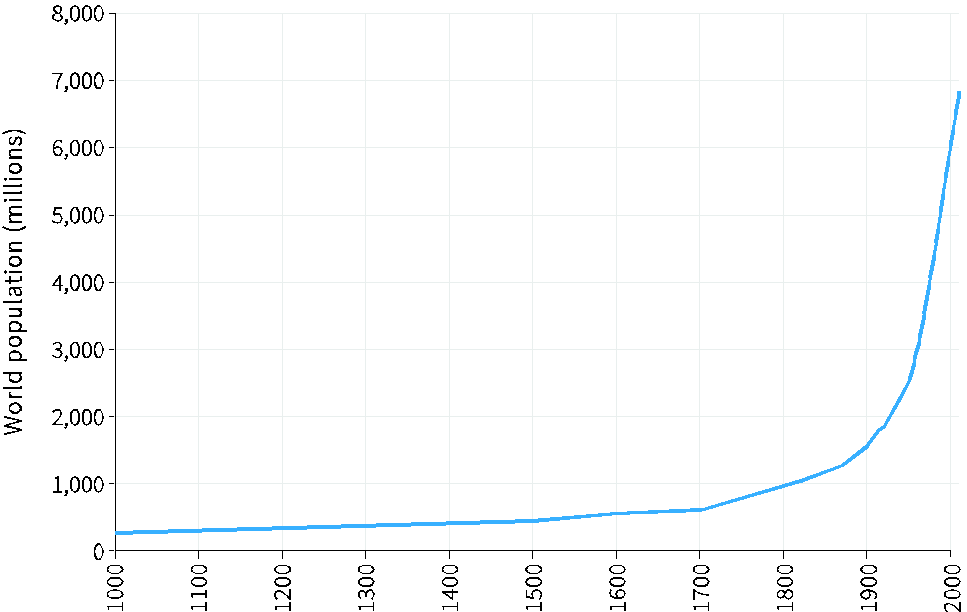
\includegraphics[width=\textwidth]{../QuestionBankImage/OUP-U1-Q10-01.png}
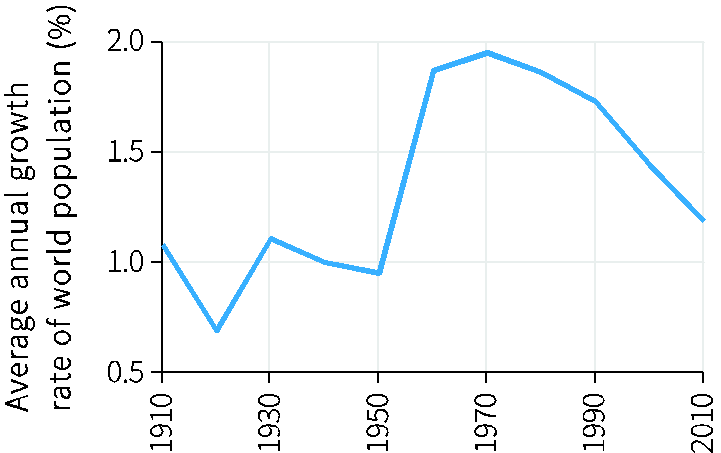
\includegraphics[width=\textwidth]{../QuestionBankImage/OUP-U1-Q10-02.png}

\begin{tasks}(1)
    \task The world population did not grow much from 1000-1700, after which the growth rate increased sharply.
        \details{The first graph shows that the population roughly doubled from 1000-1700.}
    \task The world population continues to grow at an increasing rate.
        \details{The second graph shows that the growth rate has actually fallen in recent years.}
    \task The graphs suggest that the world population will start shrinking in near-term.
        \details{While this is a possibility, the two graphs do not indicate this with certainty.}
    \task There has been a 600\% increase in the world population over the past 200 years.
        \details{From the first graph we see that the world population was around 1 billion in 1800 and nearly 7 billion in 2000. This is a 600\% increase in 200 years.}
\end{tasks}

\Question Which of the following does not lead to higher GDP?
\answer{A}

\begin{tasks}(1)
    \task Wealth transfers from the rich to the poor, which lead to higher income equality.
        \details{Equality matters for people’s wellbeing. However, it is not included in a nation’s GDP.}
    \task Higher government expenditure on education.
        \details{GDP includes the goods and services produced by the government, such as education, national defence, and law enforcement.}
    \task Rebuilding and reopening an abandoned shopping mall, which is immediately occupied by new businesses.
        \details{The activities of firms are counted as part of GDP.}
    \task Building a new manufacturing factory, which requires the clearing of forests.
        \details{Environmental damage is not reflected in GDP, but the building of a factory is.}
\end{tasks}

\Question The following table shows the nominal GDP (in 2015 US dollars) and the population of Japan in 2013 and 2014 (source: The World Bank). Based on this information, which of the following statements regarding GDP per capita is correct?
\answer{D}

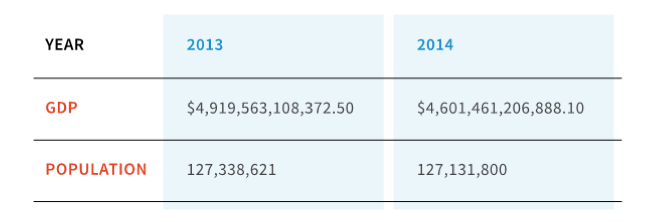
\includegraphics[width=\textwidth]{../QuestionBankImage/TEA-U1-Q1-01.png}

\begin{tasks}(1)
    \task Japan’s GDP per capita in 2013 was \$36,194.42.
        \details{The GDP per capita in 2013 was \$4,919,563,108,372.50 / 127,338,621 = \$38,633.71. \$36,194.42 is for the GDP per capita in 2014.}
    \task Japan’s GDP per capita fell by 6.74\% between 2013 and 2014.
        \details{The GDP per capita was \$38,633.71 in 2013 and \$36,194.42 in 2014. Therefore it changed by (36,194.42 – 38,633.71) / 38,633.71 = -6.31\%.}
    \task The fall in the population was enough to offset the fall in GDP, for an overall growth in GDP per capita between 2013 and 2014.
        \details{The population fell by 0.16\%. This was not enough to offset the fall in GDP of 6.47\%.}
    \task Japan’s GDP per capita fell by 6.31\% between 2013 and 2014.
        \details{The GDP per capita was \$38,633.72 in 2013 and \$36,194.42 in 2014. Therefore it changed by (36,194.42 – 38,633.71) / 38,633.71 = -6.31\%.}
\end{tasks}


\Question Which of the following statements is correct?
\answer{C}

\begin{tasks}(1)
    \task A model is an exact representation of what goes on in the economy.
        \details{A model is a simplified representation that helps to understand what happens in the economy.}
    \task A model is an economic relationship that is only represented by mathematics.
        \details{While mathematics is part of the language of economics, much of the knowledge of economics cannot be expressed in mathematics but instead requires either verbal or graphical representations.}
    \task Equilibrium is a self-perpetuating situation that does not change, unless a force for change is introduced from the outside and alters the basic data describing the situation.
        \details{This is the definition of equilibrium.}
    \task Equilibrium in GDP growth rate is when the growth rate is zero.
        \details{A non-zero rate of change can be an equilibrium if it does not change in the absence of some external force.}
\end{tasks}

\Question Production of cloth requires two inputs: L workers and R tonnes of coal. The following diagram depicts the isocost associated with production. You are also given that the wage (w) is \$20 and the price (p) of coal is \$30. Which of the following statements is correct?
\answer{A}

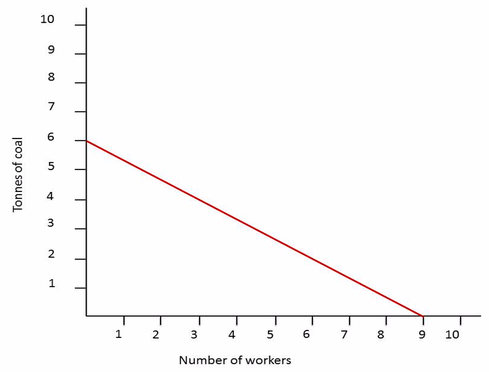
\includegraphics[width=\textwidth]{../QuestionBankImage/OUP-U2-Q8-01.png}

\begin{tasks}(1)
    \task The isocost suggests that the cost of using 6 workers and 2 tonnes of coal is the same as that of using 3 workers and 4 tonnes of coal.
        \details{(6, 2) and (3, 4) are both points on the same isocost line.}
    \task The slope of the isocost is -1/3.
        \details{The slope of the isocost is –w/p= – 2/3.}
    \task The cost associated with the isocost is \$120.
        \details{The cost associated with the isocost is \$180. We know this by calculating the cost of any point on the line. For example for the horizontall axis intercept (9, 0), c = 20 ×9 = \$180.}
    \task All points above the isocost would cost more than \$210.
        \details{All points above the isocost would cost more than any point on the line, which in this case is \$180 (see the answer to (c)).}
\end{tasks}

\Question In the following diagram you are given two technologies, A and B, which can produce 100 metres of cloth. Technology A uses 1 worker and 4 tonnes of coal, while technology B uses 4 workers and 2 tonnes of coal. The diagram also depicts three examples of isocosts, NM, GF and JH. The wage cost and the price of coal are denoted by wand p, respectively. In case 1, the wage cost and the price of coal are (w, p) = (20, 10), while in case 2, (w, p) = (10, 20). Which of the following statements is correct?
\answer{B}

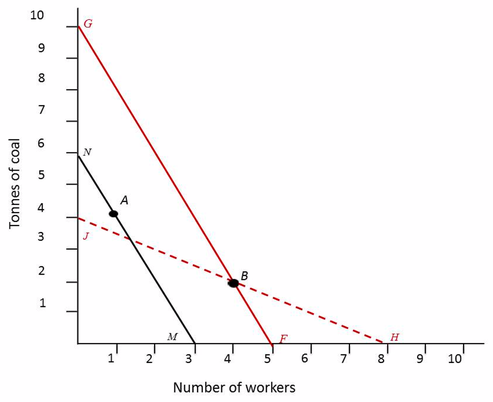
\includegraphics[width=\textwidth]{../QuestionBankImage/OUP-U2-Q11-01.png}

\begin{tasks}(1)
    \task Technology B would be chosen in both cases 1 and 2.
        \details{Isocosts NM and GF correspond to case 1 while isocost JH corresponds to case 2. In case 1, the isocost NM going through A is lower than the isocost GF going through B (due to lower total cost). This implies that A would be chosen instead of B in case 1.}
    \task Technology A would be chosen in case 1 while technology B would be chosen in case 2.
        \details{Isocosts NM and GF correspond to case 1 while isocost JH corresponds to case 2. In case 1 the lower isocost goes through A, implying that A would be chosen. Similarly in case 2, isocost JH would be lower than the corresponding isocost that would go through A, and therefore B would be chosen.}
    \task Technology B would be chosen in case 1 while technology A would be chosen in case 2.
        \details{Isocosts NM and GF correspond to case 1 while isocost JH corresponds to case 2. In case 1 technology A would be chosen, while in case 2 technology B would be chosen.}
    \task Technology B would be cheaper under case 1 than under case 2.
        \details{Under case 1 the cost of technology B is c = (\$20 × 4) + (\$10 × 2) = \$100. Under case 2 the cost is c = (\$10 × 4) + (\$20 × 2) = \$80. Therefore technology B is cheaper under case 2.}
\end{tasks}



\Question Which of the following statements regarding the Malthusian model are correct when there is a positive one-off technological shock (such as an improved seed)?
\answer{C}

\begin{tasks}(1)
    \task There is an immediate and permanent rise in the average product of labour.
        \details{A key assumption of the Malthusian model is the diminishing average product of labour as population rises.}
    \task The population initially rises but then falls to the pre-technological shock level.
        \details{The population settles at a higher level as a result of the positive technological shock.}
    \task Income initially rises but then falls to the subsistence level in equilibrium.
        \details{Subsistence level is the level at which there is no population growth. This is the equilibrium.}
    \task Malthus’ Law states that an increase in productivity will result in both increased population and wages in the long run.
        \details{Malthus’ Law states that an increase in productivity will result in a larger population but not increased wages in the long run.}
\end{tasks}

\Question Which of the following is an economic rent?

\answer{C}
\begin{tasks}(1)
    \task The amount you pay your landlord for the use of an apartment.
        \details{This is the rent as used in everyday language. Economic rent is something you would like to get and not something you have to pay.}
    \task The amount you pay to hire a car for a weekend.
        \details{An economic rent is what you earn above the next best alternative, which in this case may be the additional earnings compared to subletting the land to someone else at the same rate.}
    \task The extra profit that a successful innovator makes on bringing a new product to the market before its competitors.
        \details{This particular form of economic rent is called an innovation rent, where profits are made in excess of those offered by the next best alternative due to the adoption of new technology.}
    \task The extra profit that a firm makes when it doubles in size and there are no changes to costs or the price for each unit of its output.
        \details{This would be the normal profit you can earn in return for hard work. An economic rent is what you earn over and above the next best option, for example working really hard in another job.}
\end{tasks}


\end{Exercise}

\end{document}
